%beamer

%\PassOptionsToClass{handout}{beamer}


% \newboolean{handoutmode}
% \setboolean{handoutmode}{false}
%\newcommand{\handoutmode}{}

%% LaTeX-Beamer template for KIT design
%% by Erik Burger, Christian Hammer
%% title picture by Klaus Krogmann
%%
%% version 2.1
%%
%% mostly compatible to KIT corporate design v2.0
%% http://intranet.kit.edu/gestaltungsrichtlinien.php
%%
%% Problems, bugs and comments to
%% burger@kit.edu
\ifdefined \handoutmode
\documentclass[18pt, handout]{beamer}
\else
\documentclass[18pt]{beamer}
\fi

\usepackage[T1]{fontenc}
\usepackage[utf8]{inputenc}

\usepackage{../preamble/templates/beamerthemekit}

\usepackage[vlined]{algorithm2e}  %possible: noend, noline, ...
\usepackage{amssymb}
\usepackage{amsmath}
\usepackage{wasysym}
\usepackage{graphicx}
%\usepackage{hyperref}
\usepackage[export]{adjustbox}
\usepackage{wrapfig}
\usepackage{colortbl}
\usepackage{tikz}
\usetikzlibrary{matrix}
\usetikzlibrary{arrows.meta}
\usetikzlibrary{automata}
\usetikzlibrary{tikzmark}
\graphicspath{{images/}}
%\usepackage[colorlinks=true,urlcolor=blue,linkcolor=blue]{hyperref}
\usepackage[outline]{contour}
\usepackage{cancel}
\usepackage[warn]{textcomp}
\usepackage{multicol}
\usepackage{tabularx}
\usepackage{xcolor}
\usepackage{hhline}
\usepackage{environ}
\usepackage{calc}
\usepackage{bm}
\usepackage{xspace} % for \xspace command
\usepackage{varwidth}
\usepackage{csquotes}

\newcommand{\mycomment}[1]{}

%%%% CONFIG

\input{../preamble/config.tex}

%%%% CONFIG END

%\renewcommand{\SS}{\iffontchar\font"1E9E \symbol{"1E9E}\else SS\fi} % SHAME ON YOU, LATEX!
\newcommand{\TM}{\text{$\mbox{}^\text{\tiny TM}$}}
\newcommand{\pluseq}{\mathrel{+}=}
\newcommand{\pp}{\operatorname{++}} 
\newcommand{\mm}{\operatorname{--\mbox{\:}--}}
\newcommand{\minuseq}{\mathrel{-}=}
\newcommand{\asteq}{\mathrel{*}=}
\newcommand{\muleq}{\asteq}
\renewcommand{\mod}{\mathop{\textbf{mod}}} 
\renewcommand{\div}{\mathop{\textbf{div}}}
\newcommand{\N}{\mathbb{N}} 
\newcommand{\R}{\mathbb{R}}
\newcommand{\Z}{\mathbb{Z}}
\newcommand{\E}{\mathbb{E}}
\renewcommand{\P}{\mathbb{P}}
\newcommand{\BB}{\mathbb{B}} % \B already exists
\newcommand{\NP}{\ensuremath{\mathcal{N\hspace{-1.5pt}P}}}
\newcommand{\Oh}[1]{\mathcal{O}\!\left(#1\right)}
\renewcommand{\O}{\mathcal{O}}
\newcommand{\Om}[1]{\Omega\!\left(#1\right)}
\newcommand{\Th}[1]{\Theta\!\left(#1\right)}

\newcommand{\realTilde}{\textasciitilde\xspace}
\renewcommand{\qedsymbol}{\textcolor{black}{\openbox}}

\newcommand{\size}[1]{\ensuremath{\left\lvert #1 \right\rvert}}
\newcommand{\set}[1]{\left\{#1\right\}}
\newcommand{\tuple}[1]{\left(#1\right)}

\newcommand*{\from}{\colon}

\newcommand{\morescalingdelimiters}{   % for proper \left( \right) typography
	\delimitershortfall=0pt  % formerly: 0pt  
	\delimiterfactor=1
}
% todo later
%\delimitershortfall=0pt  % for proper \left( \right) typography
%\delimiterfactor=1

% --- \frameheight constant ---
\newlength\fullframeheight
\newlength\framewithtitleheight
\setlength\fullframeheight{.92\textheight}
\setlength\framewithtitleheight{.86\textheight}

\newlength\frameheight
\setlength\frameheight{\fullframeheight}

\let\frametitleentry\relax
\let\oldframetitle\frametitle
\def\frametitle#1{\global\def\frametitleentry{#1}\if\relax\frametitleentry\relax\else\setlength\frameheight{\framewithtitleheight}\fi\oldframetitle{#1}}

% --- \frameheight constant end ---

\def\·{\cdot}
\def\*{\cdot}
\def\<{\langle}
\def\>{\rangle}


\newcommand{\zB}{z.\,B.\@\xspace}
\newcommand{\ZB}{Z.\,B.\@\xspace}

\newcommand{\ceil}[1]{\left\lceil#1\right\rceil}
\newcommand{\floor}[1]{\left\lfloor#1\right\rfloor}
\newcommand{\abs}[1]{\left|#1\right|}
\newcommand{\Matrix}[1]{\begin{pmatrix} #1 \end{pmatrix}}
\newcommand{\braced}[1]{\left\lbrace #1 \right\rbrace}
\newcommand{\llist}[1]{\langle #1 \rangle}
\newcommand{\Mid}{\;\middle|\;}

\let\after\circ

\newcommand{\entspr}{\ensuremath{\mathrel{\hat{=}}}\xspace}

\def\~~>{\ensuremath{\rightsquigarrow}}  % FuCKING FINALLY! :D

% "something" placeholder. Useful for repairing spacing of operator sections, like `\sth = 42`.
\def\sth{\vphantom{.}}

\def\fract#1/#2 {\frac{#1}{#2}}  % ! TRAILING SPACE is CRUCIAL!
\def\dfract#1/#2 {\dfrac{#1}{#2}} % ! Trailing space is crucial!

\newcommand{\tight}[1]{{\renewcommand{\arraystretch}{0.76} #1}}
\newcommand{\stackedtight}[1]{{\renewcommand{\arraystretch}{0.76} \begin{matrix} #1 \end{matrix}} }
\newcommand{\stacked}[1]{\begin{matrix} #1 \end{matrix} }
\newcommand{\casesl}[1]{\delimitershortfall=0pt  \left\lbrace\hspace{-.3\baselineskip}\begin{array}{ll} #1 \end{array}\right.}
\newcommand{\casesr}[1]{\delimitershortfall=0pt  \left.\begin{array}{ll} #1 \end{array}\right\rbrace}
\newcommand{\caseslr}[1]{\delimitershortfall=0pt  \left\lbrace\begin{array}{ll} #1 \end{array}\hspace{-.3\baselineskip}\right\rbrace}

\def\q#1uad{\ifnum#1=0\relax\else\quad\q{\the\numexpr#1-1\relax}uad\fi}
% e.g. \q1uad = \quad, \q2uad = \qquad etc.

\newcommand{\qqquad}{\q3uad}


\def\indentstring{}
\def\§#1{\def\indentstring{#1}#1}
\def\.{{$\hphantom{\text{\indentstring}}$}}


\newcommand{\impl}{\ifmmode\ensuremath{\mskip\thinmuskip\Rightarrow\mskip\thinmuskip}\else$\Rightarrow$\xspace\fi}  
\newcommand{\Impl}{\ifmmode\implies\else$\Longrightarrow$\xspace\fi}

\newcommand{\gdw}{\ifmmode\mskip\thickmuskip\Leftrightarrow\mskip\thickmuskip\else$\Leftrightarrow$\xspace\fi}
\newcommand{\Gdw}{\ifmmode\iff\else$\Longleftrightarrow$\xspace\fi}

\newcommand{\symbitemnegoffset}{\hspace{-.33\baselineskip}}
\newcommand{\implitem}{\item[\impl\symbitemnegoffset]}
\newcommand{\Implitem}{\item[\Impl\symbitemnegoffset]}


\newcommand{\forcenewline}{\mbox{}\\}

\newcommand{\bfalert}[1]{\textbf{\alert{#1}}}
\let\elem\in   % I'm a Haskell freak. Don't judge me. :P


\newenvironment{threealign}{%
	\[
	\begin{array}{r@{\ }c@{\ }l}
}{%
	\end{array}	
	\]
}


\makeatletter
% Provides color if undefined.
\newcommand{\colorprovide}[2]{%
	\@ifundefinedcolor{#1}{\colorlet{#1}{#2}}{}}
\makeatother



%\pgfdeclarelayer{background}
%\pgfdeclarelayer{foreground}
%\pgfsetlayers{background,main,foreground}

\colorprovide{lightred}{red!30}
\colorprovide{lightgreen}{green!40}
\colorprovide{lightyellow}{yellow!50}
\colorprovide{beamerlightred}{lightred}
\colorprovide{beamerlightgreen}{lightgreen}
\colorprovide{beamerlightyellow}{lightyellow}
\colorprovide{fullred}{red!60}
\colorprovide{fullgreen}{green}
\definecolor{darkred}{RGB}{115,48,38}
\definecolor{darkgreen}{RGB}{48,115,38}
\definecolor{darkyellow}{RGB}{100,100,0}

\only<handout:0>{\colorlet{adaptinglightred}{beamerlightred}}
\only<handout:0>{\colorlet{adaptinglightgreen}{beamerlightgreen}}
\only<handout:0>{\colorlet{adaptinglightyellow}{beamerlightyellow}}
\only<beamer:0>{\colorlet{adaptinglightred}{lightred}}
\only<beamer:0>{\colorlet{adaptinglightgreen}{lightgreen}}
\only<beamer:0>{\colorlet{adaptinglightyellow}{lightyellow}}
\only<handout:0>{\colorlet{adaptingred}{lightred}}
\only<beamer:0>{\colorlet{adaptingred}{fullred}}
\only<handout:0>{\colorlet{adaptinggreen}{lightgreen}}
\only<beamer:0>{\colorlet{adaptinggreen}{fullgreen}}

\colorlet{checkgreen}{green!80}
\colorlet{crashred}{fullred}
\colorprovide{myalertcolor}{red}
\colorlet{alertcolor}{myalertcolor}

\definecolor{kwblue}{rgb}{0.3,0.3,1}
\definecolor{strcolor}{RGB}{48,115,38}

\newcommand{\str}[1]{\shorthandoff{"}\textcolor{strcolor}{\text{"{}#1"{}}\shorthandon{"}}}

\newcommand{\gray}[1]{\textcolor{gray}{#1}}

\newcommand{\MyKwSty}[1]{\textcolor{kwblue}{\textbf{#1}}}
\SetKwSty{MyKwSty}

\SetArgSty{textnormal} % to end conditional italics madness

\newcommand{\MyCommentSty}[1]{\emph{\gray{#1}}}
\SetCommentSty{MyCommentSty}

\SetKwComment{Comment}{// }{}

\newcommand{\LComment}[1]{\Comment*[h]{#1}}
\newcommand{\RComment}[1]{\quad \Comment*[h]{#1}}



\SetKwBlock{KwFunc}{function}{}
\SetKwBlock{KwProc}{procedure}{}
\newcommand{\Function}[2]{\KwFunc({#1}){#2}}
\newcommand{\Procedure}[2]{\KwProc({#1}){#2}}
\SetKwBlock{KwEmptyBlock}{}{}
\newcommand{\EmptyBlock}[1]{\KwEmptyBlock(){#1}}

% Binary operator keywords (small surrounding spaces)
\newcommand{\SetKwBin}[2]{
	\expandafter\newcommand\csname #1\endcsname{\ensuremath{\mathbin{\KwSty{#2}}}}	
}
% Relational operator keywords (bigger surrounding spaces)
\newcommand{\SetKwRel}[2]{
	\expandafter\newcommand\csname #1\endcsname{\ensuremath{\mathrel{\KwSty{#2}}}}	
}
% Directive keywords (trailing space)
\newcommand{\SetKwDir}[2]{
	\expandafter\newcommand\csname #1\endcsname{\ensuremath{\mathop{\KwSty{#2}}}}		
}

\DontPrintSemicolon
%\SetKwSwitch{Switch}{Case}{Other}{switch on}{}{}{else}{}{}

%\newcommand{\SwitchCase}[2]{\KwSty{case} #1 \KwOf\EmptyBlock{#2}}
%\newcommand{\case}[2]{#1:\EmptyBlock{#2}}
\SetKwDir{KwAssert}{assert}
\SetKwDir{KwInvariant}{invariant}
\SetKwRel{KwStep}{step}
\SetKwRel{KwDownto}{downto}	
\SetKwDir{KwArrayOf}{array of\,}
\SetKwDir{KwArray}{array}
\let\KwTo\undefined
\SetKwRel{KwTo}{to}
\SetKwRel{KwOf}{of}
\let\KwInput\KwIn
\let\KwIn\undefined
\SetKwRel{KwIn}{in}
\SetKwRel{KwInto}{into}
\SetKwDir{KwNot}{not}
\SetKwRel{KwIs}{is}
\SetKwRel{KwAnd}{and}
\SetKwRel{KwOr}{or}
\SetKwBin{KwMod}{mod}
\SetKwBin{KwDiv}{div}
\SetKwDir{KwContinue}{continue}
\SetKwDir{KwBreak}{break}
\SetKwDir{KwThrow}{throw}
\SetKw{KwTrue}{true}
\SetKw{KwFalse}{false}
\SetKw{KwThis}{this}
\SetKwDir{KwNew}{new}
\SetKwRel{KwFrom}{from}
\SetKwDir{KwFor}{for}
\SetKwDir{KwEach}{each}
\SetKw{KwProcedure}{procedure}
\SetKw{KwMethod}{method}
\SetKw{KwFunction}{function}
\SetKwDir{KwPointerTo}{Pointer to}
\SetKwData{KwList}{List}
\SetKwData{KwSet}{Set}
\newcommand{\Element}{\|Element|}
\newcommand{\KwListOf}{\ensuremath{\mathop{\KwList \KwOf}}} 
\newcommand{\KwSetOf}{\ensuremath{\mathop{\KwSet \KwOf}}} 
\SetKwDir{KwDispose}{dispose}


\def\|#1|{\text{\normalfont #1}}  % | steht für senkrecht (anstatt kursiv wie sonst im math mode)

% proper math typography
\newcommand{\functionto}{\longrightarrow} 
\renewcommand{\geq}{\geqslant}
\renewcommand{\leq}{\leqslant}
\let\oldsubset\subset
\renewcommand{\subset}{\subseteq} % for all idiots out there using subset

\newcommand{\access}{\text{\textrightarrow}} 
\def\->{\access}

\let\oldemptyset\emptyset
\let\emptyset\varnothing % proper emptyset

\newcommand{\stdarraystretch}{1.20}
\renewcommand{\arraystretch}{\stdarraystretch}  % for proper row spacing in tables

\newcommand{\mailto}[1]{\href{mailto:#1}{{\textcolor{blue}{\underline{#1}}}}}
\newcommand{\urlnamed}[2]{\href{#1}{\textcolor{blue}{\underline{#2}}}}
\renewcommand{\url}[1]{\urlnamed{#1}{#1}}

\newcommand{\hanging}{\hangindent=0.7cm}
\newcommand{\indented}{\hanging}

\newcommand{\Pros}{{\huge \protect\textcolor{adaptinggreen}{\protect\contour{black}{\raisebox{-.3pt}{$\protect\textbf{+}$}}}}\xspace}

\newcommand{\Cons}{\hspace{1pt}\protect\scalebox{0.88}[1]{\huge \protect\contour{black}{\protect\textcolor{adaptingred}{\raisebox{-1pt}{$\protect\textbf{--}$}}}}\hspace{1pt}\xspace}

\newcommand{\yop}{\textcolor{checkgreen}{\protect\contour{black}{\protect\textbf{\checked}}}\xspace}
\newcommand{\crash}{\ensuremath{\textcolor{crashred}{\protect\contour{black}{\protect\textbf{\lightning}}}}\xspace}

\newcommand{\YesCellE}[1]{\cellcolor{adaptinggreen} {#1}}
\newcommand{\YesCell}{\YesCellE{\textbf{Ja}}}
\newcommand{\NoCellE}[1]{\cellcolor{adaptingred} {#1}}
\newcommand{\NoCell}{\NoCellE{\textbf{Nein}}}


\newcommand{\TrueQuestion}[1]{
	\TrueQuestionE{#1}{}
}

\newcommand{\YesQuestion}[1]{
	\YesQuestionE{#1}{}
}

\newcommand{\FalseQuestion}[1]{
	\FalseQuestionE{#1}{}
}

\newcommand{\NoQuestion}[1]{
	\NoQuestionE{#1}{}
}

\newcommand{\DependsQuestion}[1]{
	\DependsQuestionE{#1}{}
}

\newcommand{\QuestionVspace}{\vspace{4pt}}
\newcommand{\QuestionParbox}[1]{\begin{varwidth}{.85\linewidth}#1\end{varwidth}}
\newcommand{\ExplanationParbox}[1]{\begin{varwidth}{.99\linewidth}#1\end{varwidth}}
\colorlet{questionlightgray}{gray!23}
\let\defaultfboxrule\fboxrule

% #1: bg color
% #2: fg color short answer
% #3: short answer text
% #4: question
% #5: explanation
\newcommand{\GenericQuestion}[5]{
	\setlength\fboxrule{2pt}
	\only<+|handout:0>{\hspace{-2pt}\fcolorbox{white}{questionlightgray}{\QuestionParbox{#4} \quad\textbf{?}}}
	\visible<+->{\hspace{-2pt}\fcolorbox{white}{#1}{\QuestionParbox{#4} \quad\textbf{\textcolor{#2}{#3}}} \ExplanationParbox{#5}} \\
	\setlength\fboxrule{\defaultfboxrule}
}

% #1: Q text
% #2: Explanation
\newcommand{\TrueQuestionE}[2]{
	\GenericQuestion{adaptinglightgreen}{darkgreen}{Wahr.}{#1}{#2}
}

% #1: Q text
% #2: Explanation
\newcommand{\YesQuestionE}[2]{
	\GenericQuestion{adaptinglightgreen}{darkgreen}{Ja.}{#1}{#2}
}

% #1: Q text
% #2: Explanation
\newcommand{\FalseQuestionE}[2]{
	\GenericQuestion{adaptinglightred}{darkred}{Falsch.}{#1}{#2}
}

% #1: Q text
% #2: Explanation
\newcommand{\NoQuestionE}[2]{
	\GenericQuestion{adaptinglightred}{darkred}{Nein.}{#1}{#2}
}

% #1: Q text
% #2: Explanation
\newcommand{\DependsQuestionE}[2]{
	\GenericQuestion{adaptinglightyellow}{darkyellow}{Je nachdem!}{#1}{#2}
}

\newenvironment{headframe}{\Huge THIS IS AN ERROR. PLEASE CONTACT THE ADMIN OF THIS TEX CODE. (headframe env def failed)}{}
\RenewEnviron{headframe}[1][]{
	\begin{frame}\frametitle{\ }
		\centering 
		\Huge\textbf{\textsc{\BODY} \\
		} 
		\Large {#1}
		\frametitle{\ }
	\end{frame}
}

\newcommand{\sectionheadframe}[2]{
	\section{#1}
	\begin{headframe}[#2]
		#1
	\end{headframe}	
}

\newcommand{\slideThanks}{
	\begin{frame}{Credits}
		%\begin{block}{}
			Vorgänger dieses Foliensatzes wurden erstellt von: \\[1em]
			Christopher Hommel  (urspr. Verfasser)\\
			Daniel Jungkind 
		%\end{block}
	\end{frame}
}

%% SLIDE FORMAT

% use 'beamerthemekit' for standard 4:3 ratio
% for widescreen slides (16:9), use 'beamerthemekitwide'


% \usepackage{../preamble/templates/beamerthemekitwide}

%% TITLE PICTURE

% if a custom picture is to be used on the title page, copy it into the 'logos'
% directory, in the line below, replace 'mypicture' with the 
% filename (without extension) and uncomment the following line
% (picture proportions: 63 : 20 for standard, 169 : 40 for wide
% *.eps format if you use latex+dvips+ps2pdf, 
% *.jpg/*.png/*.pdf if you use pdflatex)
\IfFileExists{images/logo.png}{
	\titleimage{logo}
}{}
\IfFileExists{images/logo.jpg}{
	\titleimage{logo}
}{}

%% TITLE LOGO

% for a custom logo on the front page, copy your file into the 'logos'
% directory, insert the filename in the line below and uncomment it

\titlelogo{empty}

% (*.eps format if you use latex+dvips+ps2pdf,
% *.jpg/*.png/*.pdf if you use pdflatex)

%% TikZ INTEGRATION

% use these packages for PCM symbols and UML classes
% \usepackage{templates/tikzkit}
% \usepackage{templates/tikzuml}

% the presentation starts here


%% Titel einfügen
\newcommand{\titleframe}{\frame{\titlepage}}

\newcounter{weeknum}

\newcounter{tasknum}
\newcounter{subtasknum}
\resetcounteronoverlays{subtasknum}
\resetcounteronoverlays{tasknum}
\let\oldthesubtasknum\thesubtasknum
\def\thesubtasknum{\ifnum\oldthesubtasknum=0\relax\else\alph{subtasknum})\fi}
\def\ThisHasSubtasks{\setcounter{subtasknum}{1337}}
\def\thetasknumminusone{\the\numexpr\thetasknum-1\relax\xspace}
\newcommand{\taskheading}[1]{\ifnum\oldthesubtasknum=1337\relax\setcounter{subtasknum}{1}\else\setcounter{subtasknum}{0}\fi\addtocounter{tasknum}{1}\textbf{Aufgabe \thetasknum\thesubtasknum: #1} \\}
\newcommand{\subtaskheading}[1]{\addtocounter{subtasknum}{1}\textbf{Aufgabe \thetasknum\thesubtasknum: #1} \\}
\newcommand{\solutionheading}{\textbf{Lösung zu Aufgabe \thetasknum\thesubtasknum} \\}

\setbeamertemplate{section in toc}{
	\gray{\inserttocsection} \par	
}
\setbeamertemplate{navigation symbols}{}

\newif\ifprinttableofcontents \printtableofcontentstrue
\def\notableofcontents{\printtableofcontentsfalse}
\let\notoc\notableofcontents

%% Alles starten mit \starttut{X}
\newcommand{\starttut}[1]{\setcounter{weeknum}{#1}\pdfinfo{
		/Author (\myname)
		/Title  (Algorithmen-Tutorium \mytutnumber, Woche \theweeknum)
	}\titleframe
	\ifprinttableofcontents\frame{\frametitle{Inhalt}\tableofcontents}\fi
	\mycomment{
		\AtBeginSection[]{%
			\begin{frame}{Wo sind wir gerade?}
				\tableofcontents[currentsection]
			\end{frame}\addtocounter{framenumber}{-1}
		}
	}	
}


\newcommand{\framePrevEpisode}{
	\begin{headframe}
		\mylasttimestext
	\end{headframe}
}

\newcommand{\lastframetitled}[6]{
	\frame{\frametitle{#6}
		\vspace{-#2\baselineskip}
		\begin{figure}[H]
			\centering
			\LARGE \textbf{\textsc{#5}} \\
			\vspace{.2\baselineskip}
			\includegraphics[#1]{#3}
			\vspace{-10pt}
			\begin{center}
				\small \url{#4} 
			\end{center}
		\end{figure} 
	}
}

% #1 number
% #2 title 
% #3 vspace (positive) without unit (\baselineskip)
\newcommand{\xkcdframe}[3]{
	\lastframetitled{width=.96\textwidth}{#3}{xkcd_#1}{http://xkcd.com/#1}{}{#2}
}

\newcommand{\xkcdframevert}[3]
{
	\lastframetitled{height=.96\frameheight}{#3}{xkcd_#1}{http://xkcd.com/#1}{}{#2}
}

\newif\ifisWS \isWSfalse

\def\semesterWS{\isWStrue}
\def\semesterSS{\isWSfalse}

\semesterSS

\def\semesterstring{\ifisWS WS \thisyear/\the\numexpr\nextyear-2000\relax\else SS \thisyear\fi}

\edef\nextyear{\the\numexpr\thisyear+1\relax} 

\title[Algorithmen-Tutorium \mytutnumber, Woche \theweeknum]{Algorithmen I \\[-2pt] Tutorium \mytutnumber}
\subtitle{Woche \theweeknum\ |\xspace\mydate{\theweeknum}}


\author[\myname]{{\mynamebold \; (\mailto{\mymail})}}

\institute{Institut für Theoretische Informatik}

\date{\mydate{\theweeknum}\ }



% Bibliography
% not needed here:
%\usepackage[citestyle=authoryear,bibstyle=numeric,hyperref,backend=biber]{biblatex}
%\addbibresource{templates/example.bib}
%\bibhang1em

% presentation

\setbeamercovered{transparent=1}  %min=0, max=100

% change the following line to "ngerman" for German style date and logos
\selectlanguage{ngerman}

\ifnum\thisyear=2018 \else \errmessage{Old ILIAS link inside preamble. Please update.} \fi

\newcommand{\ILIAS}{\urlnamed{https://ilias.studium.kit.edu/ilias.php?ref_id=808428&cmdClass=ilrepositorygui&cmdNode=k8&baseClass=ilrepositorygui}{ILIAS}\xspace} 

\newcommand{\Socrative}{\only<handout:0>{socrative.com $\qquad$ \~~> Student login \\ Raumname:  \mysocrativeroom\\ \medskip}}

\newcommand{\thasse}[1]{
	\ifdefined\ThassesTut #1\xspace \else\fi
}
\newcommand{\daniel}[1]{
	\ifdefined\DanielsTut #1\xspace \else\fi
}
\newcommand{\thassedaniel}[2]{\ifdefined\ThassesTut #1\else\ifdefined\DanielsTut #2\fi\fi\xspace}

\ifdefined\ThassesTut \ifdefined\DanielsTut \errmessage{ERROR: Both ThassesTut and DanielsTut flags are set. This is most likely an error. Please check your config.tex file.} \else \fi \else \ifdefined\DanielsTut \else \errmessage{ERROR: Neither ThassesTut  nor DanielsTut flags are set. This is most likely an error. Please check your config.tex file.} \fi\fi

\begin{document}
	
\starttut{7}

\begin{frame}{Schwarzes Brett}
	\begin{itemize}
		\item \textbf{Erinnerung}: Am \textbf{21.06.} statt Übungstermin \textbf{Probeklausur}! Hingehen lohnt sich!
		\item Nächstes Mal (23.06.) bin ich \textbf{nicht da} – werde aber \textbf{vertreten} von \textbf{Christopher} (dem Schöpfer der Vorlage dieser Folien \smiley). \\
		Blätter kriegt ihr vermutlich von ihm.
	\end{itemize}
\end{frame}
	
\begin{headframe}
	Eimerweise Sortieralgorithmen
\end{headframe}
	
\begin{frame}{Eimerweise Sortieralgorithmen}
	\textbf{Erinnerung: Bucketsort} 
	\begin{itemize}
		\item $n$ Elemente \textbf{beschränkter} Größe (also $\forall e : \; e \in \{a, ..., b\} $)
		\item Lege an \: $\|buckets|: \KwArray[a..b] \KwOf \KwListOf \|Element|$ \quad ($k := \abs{\|buckets|}$)
		\item Schmeiße jedes Element $e$ in seinen Eimer: $\|buckets|[e].\|pushBack|(e)$ (hinten anhängen)
		\item Am \textbf{Ende}: „Eimer“ zusammenhängen
		\implitem Array sortiert. 
		\item \textbf{Laufzeit}: $O(n+k)$
		\item \textbf{Aufpassen} bei großen/unbeschränkten $k$!
	\end{itemize}
\end{frame}

\begin{frame}{CountingSort}
	\textbf{Zahlen zählen} 
	\begin{itemize}
		\item Sagen wir jetzt ganz konkret: $n$ Zahlen $\in \{1,...,k\}$.
		\pause
		\item \textbf{Neue Idee}: \textbf{Zähle} (in einem Extra-Array), welche Zahl \textbf{wie oft vorkommt} (in $\Theta(n)$)
		\pause
		\item Bestimme dann, welche Zahl \textbf{in welchen Bereich} des sortierten Arrays gehört (in $\Theta(k)$)
		\pause
		\item Füge die Zahlen dann dort ein (in $\Theta(n)$)
		\pause
		\item Gesamtlaufzeit von \emph{CountingSort}: $O(n + k)$
	\end{itemize}
\end{frame}

\begin{frame}{CountingSort}
	\begin{exampleblock}{CountingSort}
		\begin{algorithm}[H]
			\small
			\Function{CountingSort$(A : \KwArray[1...n] \KwOf \N)$} {
				$C[1...k] := (0,...,0) : \KwArray \KwOf \N$ \LComment{das Zählerarray} \;
				$B[1...n] : \KwArray \KwOf \N$ \RComment{das sortierte Array (in VL ein Parameter)} \;
				\For{$i := 1 \KwTo n$} {
					$C[A[i]]\pp$\;
				}
				$C[0] := 1$\;
				\For{$i := 2 \KwTo k$} {
					$C[i] \pluseq C[i-1]$\;
				}
				\LComment{$C[\ell-1]$ sagt jetzt, wo in $B$ der Bereich für die Zahl $\ell \in A$ beginnt}
				
				\For{$i := 1 \KwTo n$} {
					$B\Big[C\big[A[i]-1\big]\Big] := A[i]$ \RComment{$A[i]$ in den zugehörigen Bereich einfügen}
					$C\left[A[i]-1\right]\pp$ \LComment{verschiebe Start des Bereiches um eins nach rechts}
				}
				\Return{$B$}\;
			}
		\end{algorithm}
	\end{exampleblock}
\end{frame}

\begin{frame}{CountingSort}
	\textbf{Eigenschaften}  \\
	\impl \textbf{Spezialfall} von Bucketsort: Eimer \entspr Zähler \\
	\pause
	\QuestionVspace
	\YesQuestion{Ist CountingSort stabil?} 
	\NoQuestion{Ist Countingsort in-place?}
\end{frame}

\begin{frame}{Eimerweise Sortieralgorithmen}
	\underline{Aufgabe 1: Das zählt nicht} \\
	Gegeben sei $ A \in \left( \bigcup\limits_{i=1}^{k} \left\lbrace i,\ i+\frac{1}{2} \right\rbrace\right)^n$. Gebt ein Verfahren an, mit dem $A$ in $O(n + k)$ sortiert werden kann. 
	% NICHT vereinfachen: Eigentliche Aufgabe ist, den Formalkram zu verstehen (sonst zu trivial)
\end{frame}

\begin{frame}{Eimerweise Sortieralgorithmen}
	\underline{Lösung zu Aufgabe 1} \\
	($A$ ist ein \textbf{Tupel} (da Element eines kartesischen Produktes).) \\
	Sortiere $A' := 2 \cdot A$ durch \emph{CountingSort} mit $k' := 2k+1$ und teile jeden Wert im sortierten Array wieder durch 2. \\
	\textbf{Laufzeit}: Da $|A'| = |A| = n$ in \\ 
	$O(n + k')$ = $O(n + 2k+1)$ = $O(n + k)$ 
\end{frame}

\begin{frame}{Radixsort}
	\textbf{Ein neuer Ansatz} \\
	\begin{itemize}
		\item \textbf{Geg}.: $n$ Zahlen $\in \N_0$  in Darstellung zur Basis $K$ mit jeweils $d$ Stellen pro Zahl 
		\pause
		\item \textbf{Idee}: $\forall $ Stelle von niedrigstwertig nach höchstwertig: \\ Sortiere mit \textbf{Bucketsort} (Buckets von $0$ bis $K-1$) nach \textbf{dieser} Stelle
		%\item \textbf{Idee}: Wende für die niedrigstwertige Stelle (\emph{LSD}) Bucketsort an und fahre mit der nächsthöherwertigen Stelle fort (das Intervall für \emph{BucketSort} geht hierbei jeweils von $0$ bis $K-1$)
		\pause
		\item \textbf{Warum} geht das? \\
		\pause 
		\impl \textbf{Stabilität} von Bucketsort
		\item \textbf{Laufzeit} von (LSD-)Radixsort: $O(d \cdot (n + K))$ \\
		{\small (LSD: \textbf{L}owest \textbf{s}ignificant \textbf{d}igit)}
	\end{itemize}
\end{frame}

\begin{frame}{Eimerweise Sortieralgorithmen}
	\underline{Aufgabe 2: Radixchensalat} \\
	Sortiert die folgende Liste mit \emph{LSD-Radixsort}:  $\langle 36, 78, 50, 1, 92, 15, 43, 99, 64 \rangle$
\end{frame}

\begin{frame}{Eimerweise Sortieralgorithmen}
	\underline{Lösung zu Aufgabe 2} \\[0,25cm]
	Eingabe:  $\langle 36, 78, 50, \gray{0}1, 92, 15, 43, 99, 64 \rangle$
	\\[0,25cm]
	Nach der ersten Stelle (von rechts): \\ $\langle 5\textbf{0}, \gray{0}\textbf{1}, 9\textbf{2}, 4\textbf{3}, 6\textbf{4}, 1\textbf{5}, 3\textbf{6}, 7\textbf{8}, 9\textbf{9} \rangle$
	\\[0,25cm]
	Nach der zweiten Stelle: \\ $\langle \textbf{0}1, \textbf{1}5, \textbf{3}6, \textbf{4}3, \textbf{5}0, \textbf{6}4, \textbf{7}8, \textbf{9}2, \textbf{9}9 \rangle$
\end{frame}

\begin{frame}{(LSD-)Radixsort}
	\textbf{Eigenschaften}   
	\begin{itemize}
		\item \textbf{Laufzeit}: linear (für \textbf{konstante} $d$ \textbf{und} $K$!) \\
		\pause
		(für große $d$: Verfahren in $\Theta(n \log n)$ geeigneter)
		\pause
		\item Ebenfalls \textbf{Spezialfall} von \emph{BucketSort}
		\pause
		\item ... und ebenfalls \textbf{stabil}, aber \textbf{nicht in-place}.
		\pause
		\item \emph{MSD-Radixsort} gibt's auch, wird hier nicht behandelt
	\end{itemize}
\end{frame}

\begin{frame}{Eimerweise Sortieralgorithmen}
	\underline{Aufgabe 3: Liste der bedrohten Sortierarten} \\
	Gegeben seien $n$ Zahlen im Bereich von $0$ bis $n^3 - 1$. Gebt ein Verfahren an, mit dem diese in $\Theta(n)$ sortiert werden können.
\end{frame}

\begin{frame}{Eimerweise Sortieralgorithmen}
	\underline{Lösung zu Aufgabe 3} \\
	Betrachte die Zahlen in Darstellung zur Basis $n$, d.h. jede Zahl hat in dieser Darstellung 3 Stellen. \\ 
	Wende $RadixSort$ an \impl die Zahlen werden in $\Theta(3 \cdot (n + n)) = \Theta(n)$ sortiert.
\end{frame}

\begin{frame}{Eimerweise Sortieralgorithmen}
	\underline{Aufgabe 4: PancakeSort} \\
	\mycomment{
		Für eine Familienfeier habt ihr euch großzügigerweise bereiterklärt, einen großen Stapel Pfannkuchen zu liefern. Ärgerlicherweise bemerkt ihr zu spät, dass eure Schöpfkelle ein Loch hat, so dass jedesmal eine unterschiedliche Menge Teig in der Pfanne gelandet ist -- somit ist jeder Pfannkuchen unterschiedlich groß und der Stapel sieht völlig chaotisch aus, weshalb \emph{bestimmt} die Welt untergeht. Glücklicherweise steht euch euer Vetter Donald mit Rat und Tat zur Seite, denn er ist der unbestrittene Weltmeister in der Kunst des Pfannkuchenwendens. Phänomenalerweise ist er sogar in der Lage, einen beliebig großen (Teil-)Stapel Pfannkuchen in einem Schwung komplett umzudrehen! Leider ist er seit einem Zwischenfall beim Pfannenwenderweitwurf etwas beschränkt, so dass er auf eure Anleitung angewiesen ist. Gebt ein In-place-Verfahren an, mit dem der Pfannkuchenstapel in möglichst geringer Zeit (bzgl. Anzahl der Pfannkuchen) sortiert werden kann.
	}
	Der ebenso geniale wie trinkfreudige Superbösewicht Doktor Meta ist in Feierlaune: Sein größter Widersacher Turing-Man {\small (halb Mensch, halb Turingmaschine)} hatte eine krachende Niederlage erlitten, nachdem Metas Schergen die Tintendüsen seines Schreiblesekopfes mit Sekundenkleber verstopft hatten. Für diesen überwältigenden Sieg schmeißen die großen Bösewichte dieser Welt natürlich eine grandiose Feier. Die Königsdisziplin dieses glorreichen Abends besteht darin, einen Stapel voller unterschiedlich großer Pfannkuchen der Größe nach zu sortieren – und das nur mit einem Pfannenwender und so schnell wie möglich. Dabei darf kein weiterer Platz benutzt werden, das heißt, der Stapel darf nur durch Wenden von Teilstapeln mit dem Pfannenwender in-place sortiert werden. Nach reichlichem Vollmilchgenuss ist Doktor Meta allerdings nicht mehr zurechnungsfähig und auf eure Anleitung angewiesen. Helft dem Superbösewicht, bevor er sich vor allen anderen blamiert.
\end{frame}

\begin{frame}{Eimerweise Sortieralgorithmen}
	\underline{Lösung zu Aufgabe 4} \\
	\begin{itemize}
		\item Zu Beginn sieht der Stapel so aus: [bottom...biggest...top]
		\item Wende Teilstapel [biggest..top] \LComment{Größter nach oben}
		\item Wende ganzen Stapel \LComment{Größter ganz unten}
		\item Für alle Teilstapel über dem nun korrekt einsortierten: \textbf{Wiederhole}.
		\implitem Pro Pfannkuchen höchstens 2-mal wenden \impl $O(n)$.
	\end{itemize}
	%Wende den Teilstapel bestehend aus dem größten Pfannkuchen und allen Pfannkuchen, die sich über diesem befinden (somit befindet sich der größte Pfannkuchen ganz oben). Wende im Anschluss den gesamten Stapel (nun ist der größte Pfannkuchen ganz unten). Setze dieses Verfahren in Bezug auf den restlichen unsortierten Teilstapel (über dem eben „einsortierten“ Pfannkuchen) fort. Folglich sind maximal zwei Wendungen pro Pfannkuchen nötig (die letzten zwei Pfannkuchen erfordern weniger), also läuft das Ganze in linearer Zeit.
\end{frame}



\begin{headframe}[And now for something completely different...]
	Binäre Heaps
\end{headframe}

\begin{frame}{Binäre Heaps}
	\textbf{} 
	\begin{itemize}
		\item \textbf{Binärbaum}: Baum, wobei jeder Knoten \textbf{max. zwei Kinder} hat.
		\pause
		\item Ein Baum $T$ erfüllt die \textbf{Heap-Eigenschaft} :\gdw \\ 
		$\forall v \in T : \quad parent(v) \leq v$ \\ 
		{\small (je näher an Wurzel $=$ Minimum, desto kleiner die Werte) } \\
		\textcolor{red}{\textbf{Achtung}}: Das heißt \textbf{nicht} \xcancel{\text{„T ist sortiert“}}!
		\pause
		\item Ein \textbf{binärer Heap} ist ein Binärbaum, der die Heap-Eigenschaft erfüllt.
		\pause
		\item \textbf{Wofür}? \impl (un/beschränkte) \textit{PriorityQueues}  {\small (brauchen wir später noch!)}
	\end{itemize}
\end{frame}

\begin{frame}{Binäre Heaps}
	\textbf{Implementierung} \\
	\begin{itemize}
		\item Repräsentiere binären Baum als $\KwArray[1...n]$ 
		%\pause
		\item Die Ebenen des Baumes liegen von \textbf{oben \~~> unten} und \\ von \textbf{links \~~> rechts} nacheinander im Array 
		\pause
		\item Von Knoten $j$ kriegt man \textbf{Eltern} und \textbf{Kinder} wie folgt:
	\end{itemize}
		%\item Hat man den Index $j$ eines Elementes, kann man somit leicht den Index der mit ihm verbundenen Elemente bestimmen: % <-- wollte ich umformulieren, aber LaTeX spackte aus O_o
		%\pause
		%\pause
	\begin{columns}
		\column{.4\textwidth}
			\vspace{-7\baselineskip} % [T] option doesn't even work. Fuck you, LaTeX!
			\begin{align*}
				&parent(j) = \floor{\tfrac{j}{2}} \\
				&leftChild(j) = 2j \\
				&rightChild(j) = 2j + 1
			\end{align*}
		\column[c]{.5\textwidth}
			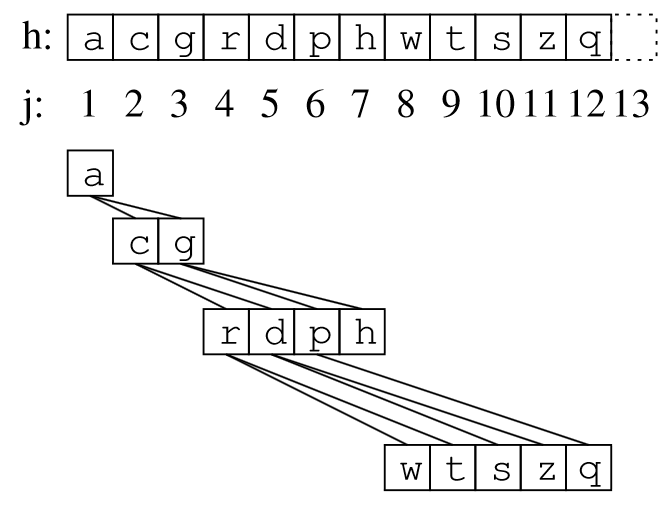
\includegraphics[height=4.7cm]{heaparray}
	\end{columns}
\end{frame}

\begin{frame}{Binäre Heaps}
	\textbf{Einfügen von Elementen (insert)} 
	\begin{itemize}
		\item Setze Element $e$ in die \textbf{unterste} Ebene, so weit \textbf{rechts} wie möglich
		\pause
		\item Heap-Eigenschaft \textbf{fixen}: mit \emph{siftUp} \\
		Vertausche $e$ solange mit seinem Parent, bis wieder erfüllt
		\pause
		\item Laufzeit: $O(\log n)$
	\end{itemize}
\end{frame}

\begin{frame}{Binäre Heaps}
	\textbf{Entfernen des Minimums (deleteMin)}
	\begin{itemize}
		\item Einfach: Minimum $= A[1]$ „\textbf{oben wegnehmen}“
		\pause
		\item \textbf{Lücke schließen}: Letztes Element $u$ aus \textbf{unterster} Ebene nach oben holen ($A[1] := A[n] = u$).
		\pause
		\item Heap-Eigenschaft \textbf{fixen}: mit \emph{siftDown} \\
		Vertausche $u$ solange mit dem jew. \textbf{kleinsten} Kind, bis wieder erfüllt
		\pause
		\item Laufzeit: $O(\log n)$
		\pause
	\end{itemize}
	\forcenewline
	\textbf{Minimum abfragen (min)}
	\begin{itemize}
		\item \Return{$A[1]$}
		\item Laufzeit: $O(1)$
	\end{itemize}
\end{frame}

\begin{frame}{Binäre Heaps}
	\textbf{Aufbau aus einem chaotischen Array (buildHeap)} 
	\begin{itemize}
		\item Haben chaotisches Array $A$, wollen \textbf{Heapstruktur} auf $A$ herstellen
		\implitem Systematisch richtigrum tauschen: \\
		\lForEach{$\text{Ebene} \in \text{Zweittiefste ... Oberste}$}{} % ftfs, I don't want to start an algo environment here
		\quad \lFor{$elem \in \text{Ebene} \KwFrom right \KwTo left$}{}
		\qquad \lIf{elem \text{too high}}{siftDown($elem$)}
		%\item Vorgehen: Gehe die Ebenen von der Zweitniedrigsten bis zur Obersten durch und tausche größere Elemente nach unten durch (mit „sift-down“)
		\pause
		\item Klingt nach $O(n \log n)$, aber Vorlesung sagt: \\
		\textbf{Laufzeit} $O(n)$
	\end{itemize}
\end{frame}

\iffalse
\begin{frame}{Binäre Heaps}
	\textbf{Adressierbare Heaps} \\[0,125cm]
	\begin{itemize}
		\item Vorhaben: Ermögliche die Änderung des Wertes eines Elementes (d.h. nach der Wertänderung wird das Element an seine neue Position hoch- bzw. runtergetauscht)
		\pause
		\item Problem: Wenn Elemente ihre Position im Array (und somit im Speicher) ständig ändern, können sie nicht beständig adressiert werden
		\pause
		\item Lösung: Halte nicht die Elemente selbst, sondern Referenzen auf diese Elemente in der Datenstruktur
	\end{itemize}
\end{frame}
\fi

\begin{frame}{Haufenweise Sortieralgorithmen}
	\textbf{Heapsort} 
	\begin{itemize}
		\item buildHeap($A$) \qquad in $O(n)$ 
		\item $n$-mal: \quad deleteMin() \qquad jeweils in $O(\log n)$ \\
		\pause
		Nach jedem deleteMin() wird ein \textbf{Platz hinten frei}: Schmeiß es \textbf{dorthin}! (\impl liefert \textbf{absteigende} Sortierung)
		\visible<2->{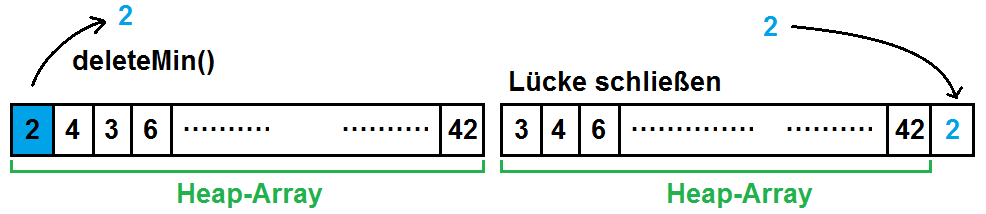
\includegraphics[width=.9\textwidth]{heapsort-inplace}}
		\pause
		\implitem \textbf{Gesamt-Laufzeit}: $O(n \log n)$ \\
		\Cons \textbf{nicht} stabil \quad (wg. siftUp/Down) \\
		\Pros in-place  \\
		\Pros Cache-effizient
	\end{itemize}
\end{frame}



\begin{headframe}[– Literally –]
	Sorting Algorithms
\end{headframe}

\begin{frame}{Sorting Algorithms}
	\textbf{Sortiere} Mergesort, Radixsort, Heapsort, InsertionSort, SelectionSort, CountingSort, Quicksort {\small (mit partition)}, (simples) Bucketsort nach \textbf{Stabilität}. \\
	\pause
	\forcenewline
	\centering
	\begin{tabular}{m{.3\linewidth} | m{.2\linewidth} |}
		\hline
		InsertionSort \newline 
		SelectionSort \newline
		Mergesort \newline
		CountingSort \newline
		Bucketsort \newline
		Radixsort & \YesCell \\
		\hline
		Heapsort \newline
		Quicksort & \NoCell \\
		\hline
	\end{tabular}
\end{frame}

\begin{frame}{Sorting Algorithms}
	\textbf{Sortiere} Mergesort, Radixsort, Heapsort, InsertionSort, SelectionSort, CountingSort, Quicksort {\small (mit partition)}, (simples) Bucketsort nach \textbf{Cache-Effizienz}. \\
	\pause
	\forcenewline
	\centering
	\begin{tabular}{m{.3\linewidth} | m{.2\linewidth} |}
		\hline
		InsertionSort \newline 
		SelectionSort \newline
		Heapsort \newline
		CountingSort \newline
		Quicksort & \YesCell \\
		\hline
		Bucketsort \newline
		Mergesort \newline
		Radixsort & \NoCell \\
		\hline
	\end{tabular}
\end{frame}

\begin{frame}{Sorting Algorithms}
	\textbf{Sortiere} Mergesort, Radixsort, Heapsort, InsertionSort, SelectionSort, CountingSort, Quicksort {\small (mit partition)}, (simples) Bucketsort nach \textbf{Platzverbrauch}. \\
	\pause
	\forcenewline
	\centering
	\begin{tabular}{m{.55\linewidth} | m{.15\linewidth} }
		\hhline{=|=}
		InsertionSort \newline 
		SelectionSort \newline
		Mergesort (ohne Rekursionsoverhead) \newline
		Quicksort (ohne Rekursionsoverhead) & $O(1)$ \\
		\hline
		Heapsort & $O(n)$ \\
		\hhline{=|=}
		CountingSort \newline 
		Bucketsort & $O(n+k)$ \\
		\hhline{=|=}
		Radixsort & $O(n+K)$ \\
		\hhline{=|=}
	\end{tabular}
\end{frame}

\begin{frame}{Sorting Algorithms}
	\textbf{Sortiere} Mergesort, Radixsort, Heapsort, InsertionSort, SelectionSort, CountingSort, Quicksort {\small (mit partition)}, (simples) Bucketsort nach \textbf{Worst-Case-Laufzeit}. \\ 
	\pause
	\forcenewline
	\begin{columns}
		\column{.45\textwidth}
		\begin{tabular}{m{.4\linewidth} | m{.3\linewidth} }
			\hhline{=|=}
			Mergesort \newline
			Heapsort & $O(n \log n)$ \\
			\hline
			Quicksort \newline 
			InsertionSort \newline 
			SelectionSort & $O(n^2)$ \\
			\hhline{=|=}
		\end{tabular}
		\column{.45\textwidth}
		\hspace{-2\baselineskip}
		\begin{tabular}{m{.37\linewidth} | m{.47\linewidth} }
			\hhline{=|=}
			Radixsort & $O(d \cdot (n + K))$ \newline ($K$: Basis, \newline $d$: Digits)\\
			\hhline{=|=}
			Bucketsort \newline
			Countingsort & $O(n+k)$ \newline ($k$: „maxValue“) \\
			\hhline{=|=}
		\end{tabular}
	\end{columns}
\end{frame}

\begin{frame}{Sorting Algorithms}
	\textbf{Sortiere} Mergesort, Radixsort, Heapsort, InsertionSort, SelectionSort, CountingSort, Quicksort {\small (mit partition)}, (simples) Bucketsort nach \textbf{„Standard-Laufzeit“}. \\
	\pause
	\forcenewline
	\begin{columns}
		\column{.55\textwidth}
		\hspace{.2\baselineskip}
		\begin{tabular}{m{.487\linewidth} | m{.3\linewidth} }
			\hhline{=|=}
			Mergesort \newline
			Heapsort \newline 
			Quicksort (erwartet) & $O(n \log n)$ \\
			\hline 
			InsertionSort \newline 
			SelectionSort & $O(n^2)$ \\
			\hhline{=|=}
		\end{tabular}
		\column{.45\textwidth}
		\hspace{-1\baselineskip}
		\begin{tabular}{m{.37\linewidth} | m{.47\linewidth} }
			\hhline{=|=}
			Radixsort & $O(d \cdot (n + K))$ \newline ($K$: Basis, \newline $d$: Digits)\\
			\hhline{=|=}
			Bucketsort \newline
			Countingsort & $O(n+k)$ \newline ($k$: „maxValue“) \\
			\hhline{=|=}
		\end{tabular}
	\end{columns}
\end{frame}

\begin{frame}{Schönes Wochenende noch! \smiley}
	\centering
	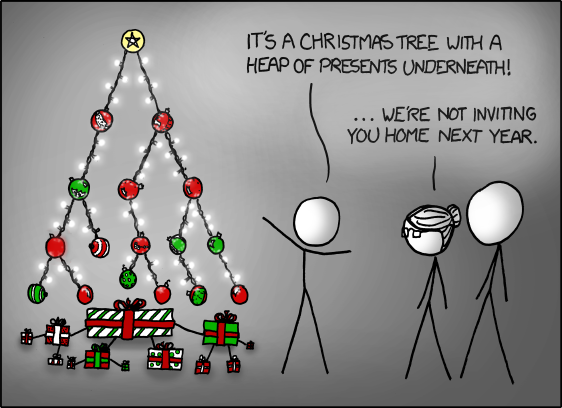
\includegraphics[width=.83\textwidth]{xkcd-835}
\end{frame}

\only<beamer:0>{\slideThanks}

\end{document}